\documentclass[11pt, twoside, a4paper]{article}
\raggedbottom

\usepackage{fontawesome5}
\usepackage{chngcntr}
\usepackage{titlesec}
\usepackage[T1]{fontenc}
\usepackage[utf8]{inputenc}
\usepackage{blindtext}
\usepackage{graphics}
\usepackage{graphicx}
\usepackage[absolute]{textpos}
\usepackage{calc}
\usepackage{csquotes}
\usepackage{scalerel}
\usepackage{xcolor}
\usepackage{hyperref}
\hypersetup{
  colorlinks=true,
  linkcolor=black,
  urlcolor=black,
  filecolor=black,
  linkbordercolor=white,
  citecolor=blue
}

\usepackage{iftex}
\usepackage{academicons}
\usepackage{amssymb,mathtools}
\usepackage[english]{babel}
\usepackage{setspace}
\usepackage{marvosym}
\usepackage{siunitx}
\usepackage{amsmath}
\usepackage{relsize}
\usepackage{amsthm}
\usepackage{fancyhdr}
\usepackage{xpatch}
\usepackage{parskip}
\usepackage{braket}
\usepackage{booktabs,dcolumn}
\usepackage{caption}
\usepackage{float}
\usepackage{xstring}
\usepackage{epstopdf}
\usepackage{url}
\usepackage{lastpage}
\usepackage{tikz}
\usepackage{textcomp}
\usepackage{epigraph}
\usepackage{shadowtext}
\usepackage{multicol}
\usepackage{pgfplots}
\pgfplotsset{compat=1.18}
\usepackage[margin=0.75in]{geometry}
\geometry{margin=1.35in}
\usetikzlibrary{arrows.meta,arrows, positioning, shapes, fit, calc}

%bibliographystyle
\usepackage[backend=biber,style=alphabetic,sorting=ynt]{biblatex}
\addbibresource{mybib.bib}

% "*" is mentioning appropriately
\DeclareUnicodeCharacter{2217}{*}
\setlength{\headheight}{14pt}

% Theorem Styles
\newtheoremstyle{mytheoremstyle}
  {5pt} % Space above
  {5pt} % Space below
  {} % Body font
  {} % Indent amount
  {\bfseries} % Theorem head font
  {.} % Punctuation after theorem head
  {5pt plus 1pt minus 1pt} % Space after theorem head
  {} % Theorem head spec (can be left empty, meaning `normal`)

\theoremstyle{mytheoremstyle}
\newtheorem{theorem}{Theorem}[section]
\newtheorem{lemma}[theorem]{Lemma}
\newtheorem{remark}[theorem]{Remark}
\newtheorem{corollary}[theorem]{Corollary}
\newtheorem{proposition}[theorem]{Proposition}
\newtheorem{hypothesis}[theorem]{Hypothesis}
\newtheorem{example}[theorem]{Example}


% Define custom titlepage style without page number but with email in the footer
\fancypagestyle{titlepage}{
    \fancyhf{} % Clear all header and footer fields
    \fancyfoot[C]{\textit{\textsuperscript{(1)} \href{mailto:abdul.halim@uni-goettingen.de}{abdul.halim@uni-goettingen.de}}} % Email address in the center of the footer
    \renewcommand{\footrulewidth}{0.4pt} % Add a line above the footer
    \renewcommand{\headrulewidth}{0pt} % No line in the header
}

\fancyhf{}
% Default footer (for pages other than the first one)
\fancyfoot[C]{Page \thepage \hspace{1pt} of \pageref{LastPage}}
\fancyhead[EC]{\texttt{Advanced Seminar on Non-commutative Geometry}}
\fancyhead[OC]{ \textsf{Abdul Halim} }
\renewcommand{\headrulewidth}{0.25pt}
\renewcommand{\footrulewidth}{0.25pt}
%title, author, email, institution name
\title{C*-algebras and K-theory for Infinite Dimensional Hilbert Manifolds}
\author{Abdul Halim\textsuperscript{(1)} \\ \textbf{Mathematisches Institut, Georg-August-Universität Göttingen}}
\date{}

\begin{document}
\pagenumbering{gobble}  % Disable page numbering for title page
    \begin{titlepage}
    \maketitle
\thispagestyle{titlepage}
    \begin{textblock*}{3cm}(0.5cm, 0.5cm) % Position: 0.5cm from the left and top
        
\includegraphics[width=2.5cm]{uni-goettingen-logo.jpg} % Adjust the width as needed on picture
    \end{textblock*}
%abstract  
\end{titlepage}
\newpage
\vspace*{\fill}
\begin{abstract}
In this research, we explore novel connections between non-commutative geometry, $C^*$-algebras, and the $K$-theory of infinite-dimensional spaces, specifically focusing on Fredholm operators. We extend the classical $K$-groups $K_0(A)$ and $K_1(A)$ for a separable $C^*$-algebra $A$, incorporating the framework of Fredholm manifolds $\mathcal{F}(H)$, where $H$ is an infinite-dimensional Hilbert space. Utilizing the Fredholm index $\operatorname{Ind}(T)$ for $T \in \mathcal{F}(H)$, we introduce new invariants in the context of twisted $K$-theory where $\operatorname{Cliff}$ is the Clifford $C^*$-algebra associated with a real quadratic form on $\mathbb{R}^n$.

We define a natural map $\phi: [T] \to \operatorname{Ind}(T)$ linking the space of Fredholm operators to the $K_1$-group $K_1(A)$, establishing a higher-dimensional Bott periodicity in non-commutative settings. Moreover, we investigate the duality between $K$-homology $K^*(X)$ and $K$-theory $K_*(C^*(X))$ within the framework of the Baum--Connes conjecture, suggesting new approaches to index theory in infinite dimensions. This research contributes to the broader understanding of non-commutative topology and extends classical theorems like the Atiyah--Singer index theorem to encompass infinite-dimensional manifolds.
\end{abstract}
\vspace*{\fill}
\newpage

%table of content
\thispagestyle{empty}
    \tableofcontents
%starting writing

\newpage
\pagenumbering{arabic}  % Restart page numbering with Arabic numerals
\setcounter{page}{1} % Start page numbering from 1
\section{Introduction}
\begin{figure}[h!]
\centering
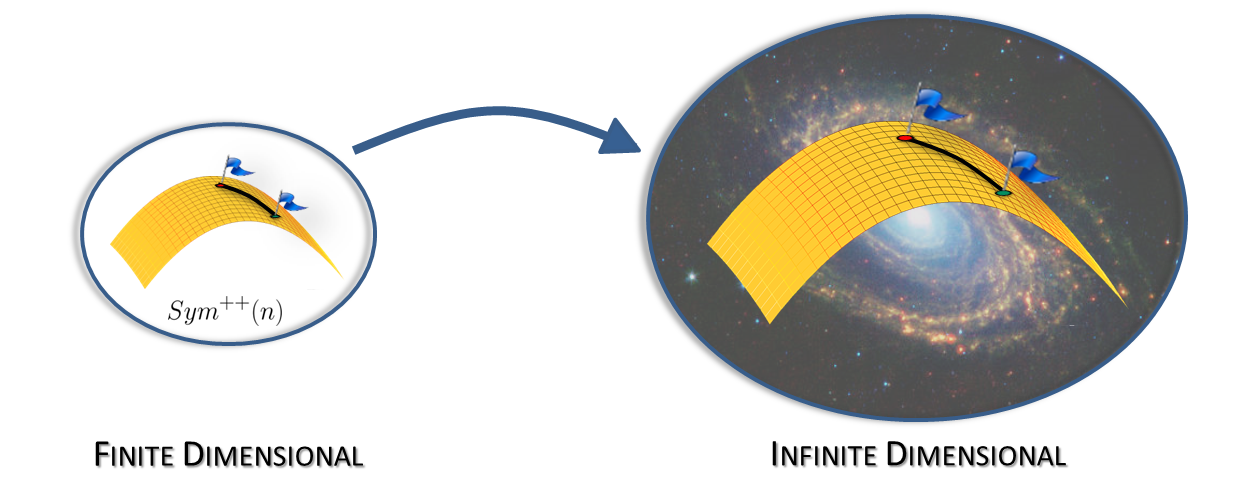
\includegraphics[width=0.7\textwidth]{manifold.png}
\caption{Idea of infinite dimensional manifold}
\end{figure}
In this research, we aim to explore the interplay between C*-algebras, K-theory, and Fredholm manifolds modeled on infinite-dimensional Hilbert spaces.

K-theory provides a unifying framework to study stable homotopy classes of vector bundles. For a compact topological space \( X \), K-theory is defined as the Grothendieck group of equivalence classes of vector bundles over \( X \). Specifically, the K-theory groups \( K_{0}(X) \) and \( K_{1}(X) \) classify stable equivalence classes of finite-dimensional vector bundles over \( X \). The group \( K_{0}(X) \) classifies even-dimensional vector bundles, while \( K_{1}(X) \) classifies odd-dimensional vector bundles.

For a C*-algebra \( A \), K-theory is adapted to a similar framework. The K-theory groups for a C*-algebra are defined as follows:
\begin{align*}
    K_{0}(A) &= \{[P] - [Q] : P, Q \text{ are projections in } A\}, \\
    K_{1}(A) &= \{[U] - [V] : U, V \text{ are unitaries in } A\}.
\end{align*}
Here, \( [P] \) and \( [Q] \) denote the classes of projections \( P \) and \( Q \) in the Grothendieck group, while \( [U] \) and \( [V] \) denote the classes of unitaries \( U \) and \( V \).

To illustrate the progression from finite-dimensional to infinite-dimensional settings, consider the following:

\begin{itemize}
    \item \textbf{Finite-Dimensional Manifolds}: For a compact manifold \( M \), the K-theory groups \( K_{0}(M) \) and \( K_{1}(M) \) capture the classification of vector bundles and their stable equivalence classes. This approach is rooted in the fundamental understanding of finite-dimensional vector bundles over \( M \).
    \item \textbf{Infinite-Dimensional Manifolds}: As we explore infinite-dimensional Hilbert spaces, we adapt the classical K-theory framework. Fredholm manifolds, which are modeled on these spaces, extend vector bundles to the infinite-dimensional context.\\ 
Their K-theory offers insights into the structure and classification of infinite-dimensional vector bundles.
\end{itemize}

The transition from finite-dimensional to infinite-dimensional contexts involves the extension of K-theory concepts to accommodate the complexities of infinite-dimensional spaces, leveraging the properties of C*-algebras and Fredholm operators to maintain coherence in classification and homotopy theory.
\section{C*-Algebras for Fredholm Manifolds}
Let \(M\) be a smooth Fredholm manifold (Hilbert Manifold) modeled on a separable infinite-dimensional Euclidean space \(\varepsilon\) with Riemannian metric \(g\). Given an augmented Fredholm filtration \(\mathcal{F}\) of \(M\) by finite-dimensional submanifolds \(\{M_{n}\}_{n=k}^{\infty}\), we associate to the triple \((M,g, \mathcal{F})\) a non-commutative direct limit C*-algebra
\begin{align}
    \mathcal{A}(M,g,\mathcal{F}) = \lim_{\substack{\to}} f(x).
\end{align}
This can play the role of the algebra of functions vanishing at infinity on the non-locally compact space \(M\). The C*-algebra \(\mathcal{A}(\varepsilon)\), as constructed by Higson-Kasparov-Trout for their Bott periodicity theorem, is isomorphic to our construction when \(M=\varepsilon\). If \(M\) has an oriented \(\operatorname{Spin}_{q}\)-structure \(1 \leq q \leq \infty\), then the K-theory of this C*-algebra is the same with a dimension shift as the topological K-theory of \(M\). Furthermore, there is a Poincaré duality isomorphism of this K-theory of \(M\)
\begin{align}
    K^{n-j}(M) \cong K_{j}^{c}(M), \quad j=0,1,
\end{align}
with the compactly supported K-homology of \(M\), just as in the finite-dimensional spin setting where \(K_{j}^{c}(M)\) denotes the dual (compactly supported) K-homology of \(M\) and \(n\) is the dimension of \(M\). This C*-algebra categorically encodes the topological properties of \(M\) and, by the Serre-Swan theorem, plays a dual role in the K-theory of \(M\):
\begin{align}
    K^{j}(M) \cong K_{j}(C_{0}(M)), \quad j=0,1,
\end{align}
where \(K^{j}(M)\) is the reduced topological K-theory of \(M\) (see \cite{eells1992}, \cite{kasparov1988}).

\section{Clifford C*-Algebras}
The other C*-algebra for a finite-dimensional \(M\) is non-commutative and constructed using the Riemannian metric \(g\). For each \(x \in M\), the tangent space \(T_{x}M\) of \(M\) is a finite-dimensional Euclidean space with inner product \(g_{x}\). Thus, we can form the complex Clifford algebra \(\operatorname{Cliff}(T_{x}M,g_{x})\). It has a canonical structure as a finite-dimensional \(\mathbb{Z}_{2}\)-graded C*-algebra. The family of C*-algebras \(\{\operatorname{Cliff}(T_{x}M,g_{x})\}_{x \in M}\) naturally forms a \(\mathbb{Z}_{2}\)-graded, C*-algebra vector bundle \(\operatorname{Cliff}(T M)\to M\), called the Clifford algebra bundle of \(M\). We then can define
\begin{align}
    \mathcal{C}(M) = C_{0}(M, \operatorname{Cliff(T M)})
\end{align}
to be the C*-algebra of continuous sections of the Clifford algebra bundle of \(M\) vanishing at infinity. This C*-algebra was used in studying the Novikov Conjecture, where he used the notation \(\mathcal{C}_{\tau} (M)\). If \(M\) is even-dimensional and has a spin structure (or, more generally, a \(\operatorname{spin}^{c}\)-structure), then this C*-algebra is Morita equivalent to \(C_{0}(M)\). (In general, \(\mathcal{C}(M)\) is Morita equivalent to \(C_{0}(T M)\).) By the Morita invariance of K-theory, it follows that
\begin{align}
    K_{j}(\mathcal{C}(M)) \equiv K_{j}(C_{0}(M)) \equiv K^{j}(M), \quad j=0,1,
\end{align}
for \(M\) odd-dimensional and spin, this is more complicated (see {\color{blue}\cite{tromba1988}}, {\color{blue}\cite{hajac1999}}).

\begin{table}[ht]
\centering
\begin{tabular}{|c|c|}
\hline
\textbf{Dimension} & \textbf{C*-Algebra} \\
\hline
1 & \(C_{0}(\mathbb{R})\) \\
\hline
2 & \(C_{0}(E^{2}, \operatorname{Cliff}(E^{2}))\) \\
\hline
\end{tabular}
\caption{Example of C*-algebras for different dimensions.}
\end{table}

\section{Generalization to Infinite-Dimensional Manifolds}
If \(M\) is an infinite-dimensional Fredholm manifold, modeled on a separable infinite-dimensional Euclidean space \(\varepsilon\), then these two constructions do not work. Both fail since compact subsets of \(M = \varepsilon\) are “thin”, i.e., contained in finite-dimensional subspaces. Thus, \(C_{0}(\varepsilon) = \{0\}\) since there are no compactly supported continuous functions on \(\varepsilon\) which are non-zero. However, the Clifford C*-algebra has been generalized by Higson-Kasparov-Trout to the case \(M = \epsilon\), by a direct limit construction that exploits an important property of Clifford algebras with respect to orthogonal sums. The component C*-algebras in the direct limit are given by
\begin{align}
    \mathcal{A}(E^{a}) = C_{0}(\mathbb{R}) \widetilde{\otimes} \mathcal{C}(E^{a}) \equiv C_{0}(\mathbb{R}) \widetilde{\otimes} C_{0}(E^{a}, \operatorname{Cliff(E^{a})}),
\end{align}
where \(\widetilde{\otimes}\) denotes the \(\mathbb{Z}_{2}\)-graded tensor product and \(C_{0}(\mathbb{R})\) is graded by even and odd functions. It is functorial with respect to inclusions of finite-dimensional subspaces, one can construct a non-commutative direct limit C*-algebra:
\begin{align}
    \mathcal{A}(\epsilon) = \lim_{\substack{\to}} \mathcal{A}(E^{a}),
\end{align}
where the direct limit is taken over all finite-dimensional subspaces \(E^{a} \subset \epsilon\) (see {\color{blue}\cite{olsen2010}}).

For a more general curved Fredholm manifold \(M\), with Riemannian metric \(g\), there does not seem to be a natural generalization of the previous constructions. Based on the above, one would be tempted to construct a direct limit C*-algebra 
\begin{align}
    \mathcal{A}(M) = \lim_{\substack{\to}} \mathcal{A}(M_{a}),
\end{align}
where the component C*-algebras should be given by
\begin{align}{\label{M_{a}}}
    \mathcal{A}(M_{a}) = C_{0}(\mathbb{R}) \widetilde{\otimes}\mathcal{C}(M_{a}),
\end{align}
and the direct limit is taken over all finite-dimensional submanifolds \(M_{a} \subset M\). The problem is that, even though the component C*-algebras have many functoriality properties, if we are given smooth isometric inclusions 
\begin{align*}
    M_{a} \subset M_{b} \subset M_{c},
\end{align*}
of finite-dimensional submanifolds of \(M\), there is no obvious way to define a commuting diagram (as there is in the Bott periodicity and Thom isomorphism cases)
\begin{center}
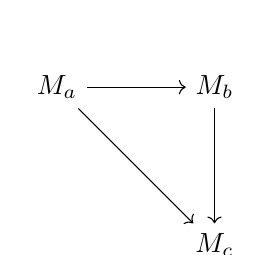
\begin{tikzpicture}[node distance=2cm, auto]
    % Nodes
    \node (A) {$M_{a}$};
    \node (B) [right of=A] {$M_{b}$};
    \node (C) [below of=B] {$M_{c}$};
    
    % Arrows
    \draw[->] (A) -- (B);
    \draw[->] (B) -- (C);
    \draw[->] (A) -- (C);
\end{tikzpicture}
\end{center}
needed to construct the corresponding direct limit (see {\color{blue}\cite{higson1997}}, {\color{blue}\cite{hajac2002}}).
\begin{theorem}
Let \( M \) be a Fredholm manifold with a Fredholm filtration
\[
\{M_{n}\}_{n=k}^{\infty},
\]
where each \( M_{n} \) is a topologically closed, finite-dimensional submanifold with
\[
\operatorname{dim}(M_{n}) = n.
\]
Then, the direct limit C*-algebra constructed as
\begin{align*}
    \mathcal{A}(M) &= \varinjlim_{n} \mathcal{A}(M_{n}), \\
    \text{where } \mathcal{A}(M_{n}) &= C_{0}(\mathbb{R}) \otimes \mathcal{C}(M_{n}),
\end{align*}
exists and provides a C*-algebra that encodes the structure of \( M \) in the infinite-dimensional setting.
\end{theorem}
\begin{proof}
First, note that each finite-dimensional submanifold \( M_{n} \) allows us to construct the C*-algebra \( \mathcal{A}(M_{n}) \) using the graded tensor product at equation ({\color{blue}\ref{M_{a}}}). Since \( \mathcal{A}(M_{n}) = C_{0}(\mathbb{R}) \widetilde{\otimes} 
 \mathcal{C}(M_{n}) \), where \( \widetilde{\otimes} \) denotes the \(\mathbb{Z}_{2}\)-graded tensor product, these C*-algebras are functorial with respect to smooth inclusions \( M_{n} \subset M_{n+1} \).

Given a Fredholm filtration \( \{M_{n}\}_{n=k}^{\infty} \), which consists of expanding finite-dimensional submanifolds, we construct the direct limit C*-algebra \( \mathcal{A}(M) \) as:
\[
\mathcal{A}(M) = \lim_{\substack{\to}} \mathcal{A}(M_{n}).
\]

For each inclusion \( M_{n} \subset M_{n+1} \), the associated maps between the C*-algebras \( \mathcal{A}(M_{n}) \) and \( \mathcal{A}(M_{n+1}) \) respect the functoriality. These maps induce a direct system of C*-algebras whose limit is a well-defined C*-algebra that reflects the structure of \( M \) in the infinite-dimensional setting.

Therefore, the direct limit construction is valid and provides a C*-algebra \( \mathcal{A}(M) \) which serves as a generalized C*-algebra capturing the properties of the Fredholm manifold \( M \) in the infinite-dimensional context. This result extends the applicability of K-theory and C*-algebras to more complex structures beyond finite dimensions.
\end{proof}
However, if the Hilbert manifold \(M\) has a Fredholm structure, then we can construct a direct limit C*-algebra by choosing an appropriate countable sequence \(\{M_{n}\}_{n=k}^{\infty}\) of expanding, topologically closed, finite-dimensional submanifolds of \(\operatorname{dim}(M_{n}) = n\). The sequence \(\{M_{n}\}_{n=k}^{\infty}\) is called a Fredholm filtration of \(M\). 
\section{Instantly}

\begin{remark}
For Fredholm manifolds \( M \), C*-algebras \( \mathcal{A}(M) \) encode the structure of \( M \) in infinite dimensions.
\end{remark}

\begin{theorem} ({\color{blue}\cite{higson2001}})
For a Fredholm manifold \( M \) with a Fredholm filtration, the direct limit C*-algebra \( \mathcal{A}(M) \) exists and encodes \( M \)'s infinite-dimensional structure.
\end{theorem}

\begin{example} ({\color{blue}\cite{trout1984}})
For \( M = E^{2} \), the C*-algebra is \( C_{0}(E^{2}, \operatorname{Cliff}(E^{2})) \).
\end{example}

\section{Objectives}
By defining new invariants and establishing a natural correspondence between Fredholm operators and the \(K_1\)-group, we seek to unveil a higher-dimensional Bott periodicity within non-commutative frameworks. Furthermore, we will explore dualities between \(K\)-homology and \(K\)-theory in the context of the Baum-Connes conjecture, thereby contributing to a deeper understanding of index theory in infinite dimensions and extending the implications of classical results, such as the Atiyah-Singer index theorem, to encompass infinite-dimensional manifolds.

\subsection{Research Goals}
The primary objectives of this research are:
\begin{itemize}
    \item Investigate the construction of C*-algebras associated with infinite-dimensional Hilbert manifolds, leveraging Fredholm structures and Fredholm filtrations.
    \item Explore the application of Clifford C*-algebras and the Thom *-Homomorphism to characterize topological and geometric properties of these manifolds.
    \item Develop a comprehensive understanding of K-theory for infinite-dimensional spaces, focusing on the relationship between C*-algebras and topological K-theory.
    \item Establish connections between non-commutative geometry and the study of infinite-dimensional manifolds through C*-algebraic techniques.
\end{itemize}

%Diagram
\subsection{Diagram Representation}

Non-commutative geometry generalizes classical spaces by replacing commutative function algebras with non-commutative \( C^* \)-algebras. A \( C^* \)-algebra \( \mathcal{A} \) is a Banach algebra with an involution satisfying
\[
\|a^* a\| = \|a\|^2 \quad \text{for all} \quad a \in \mathcal{A}.
\]
These algebras encode quantum spaces, with K-theory and Fredholm operators playing crucial roles.

Fredholm operators, defined as bounded linear operators with finite-dimensional kernel and cokernel, are linked to \( C^* \)-algebras through index theory. The index of a Fredholm operator \( T \), given by
\[
\text{ind}(T) = \dim(\ker T) - \dim(\text{coker}(T)),
\]
connects analytic data to topological information, extending the Atiyah-Singer Index Theorem to non-commutative spaces.

K-theory classifies projective modules over \( C^* \)-algebras and involves the K-groups \( K_0(\mathcal{A}) \) and \( K_1(\mathcal{A}) \). These groups encode the structure of non-commutative spaces and are essential for applying index theory to Fredholm manifolds, which generalize infinite-dimensional spaces with Fredholm operator-valued tangent spaces.

The relationships between \( C^* \)-algebras, Fredholm operators, K-theory, and Fredholm manifolds form the foundation of non-commutative geometry.

%Diagram of noncommutative geometry
\begin{figure}
\centering
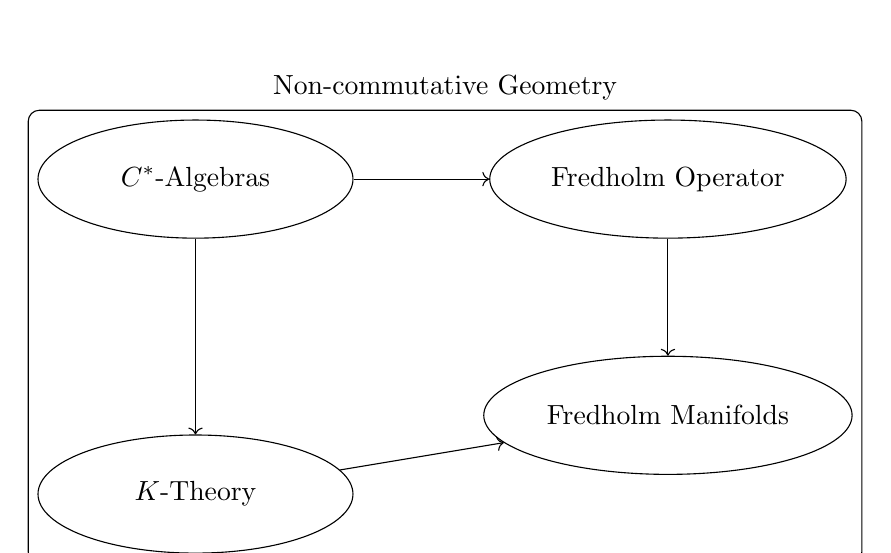
\begin{tikzpicture}[node distance=3cm, auto, scale=1, transform shape]
    % Nodes
    \node (A) [draw, ellipse, minimum width=4cm, minimum height=1.5cm] {$C^*$-Algebras};
    \node (B) [right of=A, xshift=3cm, draw, ellipse, minimum width=4cm, minimum height=1.5cm] {Fredholm Operator};
    \node (C) [below of=A, yshift=-1cm, draw, ellipse, minimum width=4cm, minimum height=1.5cm] {$K$-Theory};
    \node (D) [below of=B, yshift=0cm, draw, ellipse, minimum width=4cm, minimum height=1.5cm] {Fredholm Manifolds};

    % Box encapsulating the nodes
    \node[draw, rounded corners, fit=(A) (B) (C) (D), label=above:Non-commutative Geometry] {};
    
    % Arrows
    \draw[->] (A) -- (B);
    \draw[->] (A) -- (C);
    \draw[->] (B) -- (D);
    \draw[->] (C) -- (D);
\end{tikzpicture}
\caption{Diagram of Non-commutative Geometry}
\end{figure}

\section{Conclusion}
This research plan outlines a systematic approach to investigate the construction and properties of C*-algebras associated with infinite-dimensional Hilbert manifolds. By leveraging the theory of Fredholm manifolds and advanced algebraic techniques, we aim to deepen our understanding of the interplay between geometry, topology, and operator algebras in the infinite-dimensional setting.

\begin{hypothesis}
For a Fredholm manifold \( M \) equipped with a Fredholm filtration \( \{M_{n}\}_{n=k}^{\infty} \), where each \( M_{n} \) is a finite-dimensional submanifold with \( \operatorname{dim}(M_{n}) = n \), it is hypothesized that:

\begin{itemize}

\item \textbf{K-Theory Extension:} 
The direct limit C*-algebra \( \mathcal{A}(M) = \lim_{\substack{\to}} \mathcal{A}(M_{n}) \) encodes new K-theory invariants for \( M \), potentially revealing novel classes and extending known results from finite to infinite dimensions.

\item \textbf{Functorial Structure:} 
The functorial properties of \( \mathcal{A}(M) \) with respect to smooth inclusions of \( M_{n} \) could lead to a deeper understanding of the stability and deformation of Fredholm manifolds, potentially yielding new analytical tools.
A continuation of the hypothesis follows:

\item \textbf{Index Theory:}
The C*-algebra \( \mathcal{A}(M) \) associated with a Fredholm manifold \( M \) equipped with a Fredholm filtration could provide a framework for extending classical index theory to infinite-dimensional settings. Specifically, it is hypothesized that the direct limit structure of \( \mathcal{A}(M) \) encodes index invariants for families of Fredholm operators over \( M \), thus contributing to a broader understanding of analytical indices in non-commutative geometry.

\item \textbf{Non-commutative Geometry:}
The construction of non-commutative C*-algebras for infinite-dimensional Hilbert manifolds may reveal new connections between non-commutative geometry and classical differential geometry. This approach could lead to a deeper exploration of the topological and geometric properties of these spaces through the lens of operator algebras, enriching both fields with novel insights and computational tools.
\end{itemize}
\end{hypothesis}
This hypothesis aims to bridge the gap between finite-dimensional K-theory, non-commutative C*-algebras, and infinite-dimensional manifolds by utilizing the rich structure of Fredholm filtrations and extending classical results in new directions.

%new page issued
\newpage
% Add a new entry to the end of the Table of Contents
\addcontentsline{toc}{section}{\hspace{0.6cm}References}
% References section (not counted in page numbering)
\thispagestyle{empty} % Hide page number on this page
%printing references
\printbibliography

\end{document}